
\documentclass[a4paper,12pt,parskip=full]{scrartcl}
\usepackage[light]{kpfonts}
\usepackage{microtype}
\usepackage[ngerman]{babel}
\usepackage[utf8]{inputenc}
\usepackage{algorithm}
\usepackage[noend]{algorithmic}
\usepackage{amsmath}
\usepackage{amssymb}
\usepackage{amsthm}
\usepackage{bbm}
\usepackage{enumerate}
\usepackage{graphicx}
\usepackage{listings}
\usepackage{float}
\usepackage{color}
\usepackage{hyperref}
\usepackage{multicol}
\usepackage[right=3.5cm, left=3.5cm, top=3cm, bottom=3cm]{geometry}
\usepackage{scrlayer-scrpage}
\usepackage{array}   % for \newcolumntype macro

%\clearpairofpagestyles
 
\setkomafont{pagehead}{\scshape\footnotesize}
%\setkomafont{pagination}{}

\KOMAoptions{
   headsepline = true
}

\newcolumntype{C}{>{$}c<{$}}

\newcommand{\Fach}{Einführung in die praktische Informatik}
\newcommand{\Semester}{Wintersemester 19/20}

\ihead{\Fach{}}
\ohead{\Semester{}}

\newtheoremstyle{exercise}
  {2\topsep}   % ABOVESPACE
  {\topsep}   % BELOWSPACE
  {\normalfont}  % BODYFONT 
  {0pt}       % INDENT (empty value is the same as 0pt)
  {\bfseries \scshape} % HEADFONT
  {.\quad}         % HEADPUNCT
  {5pt plus 1pt minus 1pt} % HEADSPACE
  {}          % CUSTOM-HEAD-SPEC

\theoremstyle{exercise}
\newtheorem{exercise}{Aufgabe}
\setcounter{exercise}{-1}

\hypersetup{%
  pdftitle={Übungsaufgaben zur Klausur},%
  pdfborder={0 0 0}%
}

\definecolor{mygreen}{rgb}{0,0.6,0}
\definecolor{mygray}{rgb}{0.5,0.5,0.5}
\definecolor{mymauve}{rgb}{0.58,0,0.82}
\lstset{ %
  basicstyle=\footnotesize, 
  language=C++,
  %numbers=left,
  stepnumber=1,
  showstringspaces=false,
  breaklines=true,                 % automatic line breaking only at whitespace
  captionpos=b,                    % sets the caption-position to bottom
  commentstyle=\color{mygreen},    % comment style
  escapeinside={\%*}{*)},          % if you want to add LaTeX within your code
  keywordstyle=\color{blue},       % keyword style
  stringstyle=\color{mymauve},     % string literal style
}

\title{Übungsaufgaben zur Klausur}


\begin{document}

\begin{center}
  {\LARGE Übungsaufgaben zur Klausur} \\
\end{center}
Die Aufgaben folgen keiner speziellen Anordnung, weder
was die Schwierigkeit, noch was das Thema betrifft. Außerdem sind auch einige Aufgaben
nicht im Stil typischer \glqq{}Klausuraufgaben\grqq{}, und dienen eher dazu ausgewählte
Themen zu vertiefen.

\begin{exercise}[Kurzfragen]
\begin{enumerate}[a)]
\item Warum sind Turing-Maschinen im Zusammenhang mit dem Begriff der
  Berechenbarkeit so interessant? Was ist die Church-Turing-These?
\item Was ist das Halteproblem? Zu welcher ``Klasse'' von Problemen
  gehört es?
\item Programmiersprachen, in denen man (wenn unendlich viel Speicher
  zur Verfügung stünde) eine Turingmaschine emulieren kann, nennt man
  Turing-vollständig. Warum ist diese Eigenschaft interessant,
  bzw. was sagt das über die Programmiersprache aus?
\item Was ist eine Referenz, wie wird sie deklariert und wozu benutzt
  man sie? Warum würde man Referenzen an Stelle von Zeigern benutzen?
  Wann können Referenzen Zeiger nicht ersetzen?
\item Welche verschiedenen Anwendungsfälle haben Zeiger?
\item Was versteht man unter einem Seiteneffekt einer Funktion oder
  Methode?
\item Wann spricht man von Funktionen, wann von Methoden?
\item Welchen Vorteil hat es, Speicher dynamisch zu allokieren? Und
  wie geht das überhaupt?
\item Was heißt es, dass C++ streng typgebunden ist? Und was versteht
  man unter statischer Typisierung?
\item Was sind typische Eigenschaften funktionaler Programmierung?
  Welche Vor- und Nachteile hat funktionale Programmierung?
\item Was ist ein Konstruktor? Was ist der Default-Konstruktor? Was
  ist der Copy-Konstruktor?
\item Was ist der Destruktor?
\item Was bedeutet Sichtbarkeit im Zusammenhang mit Klassen in C++?
  Welche verschiedenen ``Sichtbarkeiten'' gibt es in C++? Wofür werden
  sie jeweils verwendet?
\item Was ist Vererbung? Gebe ein Minimalbeispiel an.
\item Erläutere grob die einzelnen Schritte die durchgeführt werden,
  um vom Quellcode zum fertigen Programm zu kommen.
\item Was ist Moore's law? Ist es immer noch gültig? Welche
  Auswirkungen hat das auf die Softwareentwicklung?
\item Was versteht man unter Overloading (deutsch: Überladen) von
  Funktionen?
\item Was versteht man unter \emph{Call by Value} und \emph{Call by
    Reference}?
\item Was versteht man unter der Signatur einer Funktion/ Methode?
\item Was ist die Rule of Three?
\item Was sind die Unterschiede zwischen einer \emph{shallow copy} und
  einer \emph{deep copy}?
\item Mittels \lstinline{using namespace std;} kann man alles aus dem
  Namensraum \lstinline{std} ``bekannt'' machen. Welche Nachteile
  könnte das haben (bspw. in größeren Projekten)?
\item Was ist eine \lstinline{friend}-Class?
\item Was macht das Schlüsselwort \lstinline{inline} vor einer
  Funktionendeklaration?
\item Was ist eine abstrakte Klasse?
\item Was ist der Unterschied zwischen öffentlicher und privater
  Vererbung?
\end{enumerate}
\begin{enumerate}[aa)]
\item Was sind (rein) virtuelle Methoden?
\item Was ist der Unterschied zwischen Overloading (Überladen) und
  Overriding (Überschreiben)?
\item Wozu verwendet man das Schlüsselwort \lstinline{template}?
\item Was ist der Unterschied zwischen \lstinline{template <class T>}
  und \lstinline{template <typename T>}?
\item Was ist \texttt{RISC}, was ist \texttt{CISC}?
\item Was ist dynamischer Polymorphismus?
\item Was ist statischer Polymorphismus?
\item Was ist ein vollständiger binärer Baum? Was ist der Unterschied
  zu einem Heap?
\item Wann ist ein Sortierverfahren stabil?
\end{enumerate}
\end{exercise}
\newpage

\begin{exercise}
Ist ein Polynom in der Form
$p(x) = a_0 + a_1 x + \dots + a_nx^n$ gegeben, so können einzelne
Werte $p(\xi)$ mit Hilfe des \emph{Horner-Schemas} berechnet werden:
\begin{align*}
  b_n &= a_n, \\
  b_k &= a_k + \xi b_{k+1} \text{ für } k = n-1, \dots, 0, \\
  p(\xi) &= b_0
\end{align*}
\begin{enumerate}[a)\ ]
\item
  Schreibe eine rekursive Funktion \lstinline{double horner(double coeffs[], int deg, double x)}, die für ein Polynom vom Grad \lstinline{deg}, dessen Koeffizienten im Array \lstinline{coeffs} stehen, das Polynom an der Stelle \lstinline{x} auswertet. \\
  Die Koeffizienten sollen dabei folgendermaßen in einem Array gespeichert werden: \\
  Für $p(x) = 3 - 2x + 3x^2 - 4x^4$ ist \lstinline|coeffs = { -4, 0, 3, -2, 3 }|
  (d.h. der höchste Koeffizient kommt zuerst). Außerdem
  ist \lstinline{deg = 4} und bspw. p(2) würde ausgewertet durch den
  Aufruf \lstinline{horner(coeffs, 4, 2) = -981 }.
  
\item Schreibe nun die Funktion aus a) iterativ. Was ist die
  Zeitkomplexität in Abhängigkeit von \texttt{n} der iterativen
  Variante?
\item[c)*] Was könnten Vorteile des Horner-Schemas sein? Warum wertet
  man das Polynom nicht einfach ``normal'' aus, indem man einfach
  $\xi$ einsetzt?
\end{enumerate}
\end{exercise}

\begin{exercise}
Schreibe eine Funktion, die ein Polynom der Form
$p(x) = a_0 + a_1 x + \dots + a_nx^n$ von der Standardeingabe liest
und die Koeffizienten $a_0, \dots, a_n$ extrahiert. \\
Bsp.: Eingabe: \texttt{2 + 2x - 3x\textasciicircum 2 + 4x\textasciicircum 3}, Ausgabe: \texttt{ \{ 2, 2, -3, 4 \} } \\
Hinweise:
\begin{itemize}
\item Der Einfachheit halber, kann davon ausgegangen werden, dass alle
  Koeffizienten einstellig sind, also dass $|a_i| \le 9$, für alle
  $i=0,\dots,n$
\item Ersetze zunächst alle '-' durch '+-' mit der Methode
  \lstinline{std::string::replace} (um bspw. im String \lstinline{s}
  alle 'a' durch 'b' zu ersetzen: \lstinline{replace(s.begin(), s.end(), 'a', 'b')} )
\item ``Splitte'' nun den String jeweils an den '+'. Du kannst
  annehmen, dass eine Funktion \lstinline{std::vector<std::string> split(const std::string &s, char delimiter)} gegeben ist, die
  einen String \lstinline{s} bei jedem Vorkommen von
  \lstinline{delimiter} aufsplittet und die einzelnen Teile in einen
  \lstinline{std::vector} schreibt (also bspw.:
  \lstinline|split("abc+def+ghi+jkl", '+') == { "abc", "def", "ghi", "jkl" }|
\item Nun kannst du den im vorherigen Schritt erstellten Vektor
  durchlaufen und die Koeffizienten extrahieren. Hier musst du nur
  aufpassen, falls ein Koeffizient 0 ist und das dazugehörige Monom
  gar nicht in der Eingabe vorkam (also bspw. $3 - 4x^2$, hier fehlt
  der Term $0x$, d.h. der Koeffizientenvektor ist hier \texttt{\{ 3,
    0, -4 \}})
\end{itemize}
\end{exercise}

\begin{exercise}
Schreibe eine Funktion \lstinline{std::vector<std::string> split(const std::string &s, char delimiter)}, die einen String
\lstinline{s} bei jedem Vorkommen von \lstinline{delimiter}
aufsplittet und die einzelnen Teile in einen \lstinline{std::vector}
schreibt (also bspw. sollte das Ergebnis von
\lstinline|split("abc+def+ghi+jkl", '+')| das hier sein: \lstinline|{"abc", "def", "ghi", "jkl" }| )
\begin{itemize}
\item Einen neuen \lstinline{std::vector}, der \lstinline{std::string}s enthält, legt man so an: \\
  \lstinline{std::vector<std::string> res;}
\item Um \lstinline{res} ein neues Element hinzuzufügen, verwende
  \lstinline{res.push_back("test")}
\item Die Funktion (siehe auch Übungsblatt 10) \\
  \centerline{ \lstinline{std::istream& getline(std::istream& is, std::string &s)} } \\
  akzeptiert auch noch einen dritten Parameter \lstinline{char delimiter} und kann auch auf \lstinline{std::stringstream}s
  operieren (um einen \lstinline{std::stringstream} aus einem String
  zu erstellen, übergibt man einfach den jeweiligen String dem
  Konstruktor).
\end{itemize}
\end{exercise}

\begin{exercise}
Implementiere die Funktion \lstinline{void reverse(std::string& s)}, die den String \lstinline{s} ``umdreht'',
also bspw. aus \texttt{Hallowelt} \texttt{tlewollaH} macht, auf die
folgenden Arten:
\begin{enumerate}[a)]
\item Implementiere die Funktion mit einer \texttt{for}-Schleife und
  der Funktion \lstinline{std::swap(char &a, char &b)}, die den Wert
  von \texttt{a} und \texttt{b} tauscht. Die \texttt{for}-Schleife
  soll dabei \emph{nicht} den ganzen String durchlaufen, sondern
  (falls \texttt{n} die Länge des Strings ist) nur von \lstinline{i = 0} bis \lstinline{i < n / 2}.
\item Implementiere die Funktion rekursiv, die Signatur der Funktion
  ändert sich dabei zu: \lstinline{std::string reverse(const std::string &s)} und die Funktion ändert nicht den ursprünglichen
  String sondern gibt das Ergebnis zurück.
\end{enumerate}
\end{exercise}

\begin{exercise}
Rechne die folgenden Zahlen um:
\begin{enumerate}[a)]
\item $11011101_2$ ins Dezimalsystem
\item $116_{10}$ ins Dualsystem
\end{enumerate}
\end{exercise}

\begin{exercise}
Gegeben seien zwei Rechtecke in einem 2D-Koordinatensystem
(jeweils parallel zu den Koordinatenachsen). Diese können eindeutig
durch Angabe der Koordinaten der linken oberen Ecke und der rechten
unteren Ecke bestimmt werden:
\begin{lstlisting}
  class Rectangle {
    public:
    double x1, y1; // linke obere Ecke
    double x2, y2; // rechte untere Ecke
  }
\end{lstlisting}
Schreibe eine Methode \lstinline{bool Rectangle::doesOverlap(const Rectangle other)}, die für ein Rechteckt prüft, ob sich seine Fläche
und die Fläche eines anderen Rechtecks überschneiden.
\end{exercise}

\begin{exercise}
\begin{enumerate}[a)]
\item Implementiere eine Klasse, die eine doppelt verkettete Liste
  repräsentiert und zumindest folgendes Interface erfüllt:
  \begin{lstlisting}
    class DLL {
      public:
      void addFirst(int value);
      int removeFirst();

      void print() const;
      void printReverse() const;

      ~DLL();
  
      private:
      struct IntListItem {
        int value = 0;
        IntListItem *next = nullptr;
        IntListItem *prev = nullptr;
      };

      IntListItem *first = nullptr;
      IntListItem *last = nullptr;
      int count = 0;
    };
  \end{lstlisting}
  Untenstehende \lstinline{main}-Funktion soll folgenden Output erzeugen: \\
  \texttt{List: 4 -> 3 -> 2 -> 1 \\
    List (reversed): 1 -> 2 -> 3 -> 4 }
  \begin{lstlisting}
    int main() {
      DLL list;
      list.addFirst(1);
      list.addFirst(2);
      list.addFirst(3);
      list.addFirst(4);

      list.print();
      list.printReverse();
  
      return 0; 
    }
  \end{lstlisting}
\item Welche Vorteile hat diese Variante gegenüber einfach verketteten
  Listen? Und gegenüber einem normalen Array? Welche Nachteile gibt
  es?
\end{enumerate}
\end{exercise}

\begin{exercise}
Gegeben sei die Turingmaschine $M$ mit den Endzuständen
$z_3$ und $z_5$, dem Startzustand $z_0$ und untenstehendem Programm.
\begin{table}[ht]
  \centering
  \begin{tabular}{C C C C C}
    \text{Zustand} & \text{Eingabe} & \text{Ausgabe} & \text{Richtung} & \text{Folgez.} \\
    \hline
    z_0 & b & b & R & z_1 \\
    z_1 & b & 0 & L & z_3 \\
    z_1 & 0 & b & R & z_2 \\
    z_2 & b & 0 & L & z_4 \\
    z_2 & 0 & b & R & z_1 \\
    z_4 & b & 0 & L & z_5 \\
  \end{tabular}
\end{table}

Die Turingmaschine berechnet die charakteristische Funktion
$\chi_M : \mathbb{N} \rightarrow \{0,1\}$ einer unbekannten Menge
$M \subseteq \mathbb{N}$, d.h.
\begin{align*}
  \chi_M(n) =
  \begin{cases}
    1 & n \in M \\
    0 & n \not\in M
  \end{cases}
\end{align*}
\begin{enumerate}[a)]
\item Ziel ist es, herauszufinden, um welche Menge $M$ es sich
  handelt. Eingabe und Ausgabe werden dabei durch eine Unärdarstellung
  codiert: $n \in \mathbb{N}$ entspricht $0^{n+1}$, d.h. $0 = 0$,
  $1 = 00$, $2=000$ etc. Die Ausgabe der Turingmaschine ist am Ende
  die Zahl, die rechts vom Schreib-Lese-Kopf steht.
\item Entwerfe nun eine Turingmaschine, welche die charakteristische
  Funktion $\chi_{M^{\mathsf{c}}}$ des Komplements
  $M^{\mathsf{c}} = \mathbb{N} \setminus M$ berechnet, d.h.
  $ \chi_{M^{\mathsf{c}}}(n) = 1 - \chi_M(n) $.
\end{enumerate}
\end{exercise}

\begin{exercise}
 Du stößt in einem Programm auf folgenden Ausschnitt:
\begin{lstlisting}
  // Pruefe, ob der Eintrag an der Stelle i, j Null ist
  if (std::abs(matrix[i][j]) < 1e-12) {
    ...
  }
\end{lstlisting}
Erkläre, warum der Code und das Kommentar darüber (auch wenn nicht
ideal formuliert) trotzdem Sinn ergeben.
\end{exercise}

\begin{exercise}
Formalisiere den Begriff Algorithmus. Welche speziellen
Typen von Algorithmen gibt es und was zeichnet sie aus? Nenne jeweils
ein Beispiel.
\end{exercise}

\begin{exercise}
Ersetze im folgenden Programmausschnitt die
\lstinline{if-else}-Konstruktion durch eine einzige möglichst
vereinfachte \lstinline{if}-Anweisung:
\begin{lstlisting}
  if (true) {
    if (x > 0) {
      if (x%2 == 0)
      std::cout << x;
    } else {
      if ((-x)%3 == 0)
      std::cout << x;
    }
  }
\end{lstlisting}
\end{exercise}

\begin{exercise}
\begin{enumerate}[a)]
\item Was macht der folgende Algorithmus?
\begin{lstlisting}
void func(int a[], int b) {
  for (int j = 1; j < b; j++)
    for (int i = j; i > 0 && a[i-1] > a[i]; i--) {
      int c = a[i];
      a[i] = a[i-1];
      a[i-1] = c;
    }
}
  \end{lstlisting}
\item Welche Laufzeit hat der Algorithmus im schlechtesten Fall?
\end{enumerate}
\end{exercise}

\begin{exercise}
\begin{enumerate}[a)]
\item Berechne die Zweierkomplementdarstellung der folgenden Zahlen:
  \begin{enumerate}[i)]
  \item -30
  \item 25
  \item 123
  \end{enumerate}

\item Rechne die folgenden Zahlen, die in Zweierkomplementdarstellung
  vorliegen, ins Dezimalsystem um:
  \begin{enumerate}[i)]
  \item 11111111
  \item 11100000
  \item 00000001
  \end{enumerate}

\item Welche Vorteile hat die Zweierkomplementdarstellung?
\end{enumerate}
\end{exercise}

\begin{exercise}
Implementiere eine Klasse, die einen Stack
modelliert. Der Typ der Werte auf dem Stack, soll durch templates
allgemein gehalten werden, d.h. die Klassendefinition sieht
folgendermaßen aus:
\begin{lstlisting}
  template <class T>
  class Stack {
    public:
    Stack(int capacity);
    ~Stack();
    bool push(T);
    T pop();

    private:
    ...
  };
\end{lstlisting}
\end{exercise}

\begin{exercise}
\begin{enumerate}[a)]
\item Erstelle eine Funktion \lstinline{double mean(const std::vector<double>& v)}, die den Mittelwert $\mathbb{E}[v]$ aller
  Einträge in dem Vektor $v$ zurückliefert:
  $$
  \mathbb{E}[v] = \frac{1}{N} \sum\limits_{i=1}^N{v_i},
  $$
  wobei $N$ die Anzahl der Einträge im Vektor angibt.
\item Erstelle eine Funktion \lstinline{double median(const std::vector<double>& v)}, die den Median aller Einträge in dem
  Vektor $v$ zurückliefert. Um den Median zu berechnen, erstelle eine
  sortierte Kopie $\tilde{v}$ von $v$ und bestimme $M(v)$ als
  $$
  M(v) =
  \begin{cases}
    \tilde{v}_{\frac{N+1}{2}} & N \text{ ungerade } \\
    \frac{1}{2} ( \tilde{v}_{\frac{N}{2}} + \tilde{v}_{\frac{N}{2}+1}
    ) & N \text{ gerade }
  \end{cases}
  $$
  wobei $N$ die Anzahl der Einträge im Vektor angibt. Beachte die
  unterschiedlichen Indizierungsstrategien (1-basiert in der Formel
  oben, 0-basiert in C++), sowie den Spezialfall, dass der Vektor leer
  ist. Benutze zum Sortieren \lstinline{std::sort(v.begin(), v.end())}.
\end{enumerate}
\end{exercise}

\begin{exercise}
\begin{enumerate}[a)]
\item Schreibe eine Funktion \lstinline{bool check_parentheses(std::string symbols)}, die für eine Zeichenkette
  \lstinline{symbols} überprüft, ob diese genau so viele öffnende
  Klammern \lstinline{'('} wie schließende \lstinline{')'}
  enthält. Die Funktion soll auch \lstinline{false} zurückgeben, wenn
  eine schließende Klammer vor einer öffnenden Klammer auftritt.
  \begin{enumerate}[i)]
  \item Verwende zunächst einfach eine \lstinline{int}-Variable um
    mitzuzählen.
  \item Verwende \lstinline{std::stack<char>}.
  \end{enumerate}
\item Kann man einen endlichen Automaten definieren, der dieselbe
  Aufgabe löst?
\end{enumerate}
\end{exercise}

\begin{exercise}
Gegeben seien folgende Zahlen:
$$ \{ 5, 8, 2, 10, 1, 3, 2, 6 \} $$
\begin{enumerate}[a)]
\item Baue aus diesen Zahlen einen Max-Heap (d.h. das größte Element
  steht in der Wurzel). Zeichne den vollständigen Baum nach jedem
  Schritt und erläutere kurz, wie das Element eingefügt wurde.
\item Lösche nun die Wurzel aus dem Baum und erläutere die dabei
  auftretende Schritte.
\item Wieviele ``Ebenen'' hat ein Heap (in Abhängigkeit der Anzahl der
  Elemente $n$)? Wie kann man daraus die Komplexität der Operation
  ``Einfügen'' ableiten?
\item Erläutere kurz die Funktionsweise von Heapsort.
\end{enumerate}
\end{exercise}

\begin{exercise}
Schreibe eine templatisierte Funktion \texttt{quicksort},
die einen \lstinline{std::vector<T>} mittels dem Quicksort-Algorithmus
sortiert. Das Pivot-Element soll dabei immer das ``mittlere'' Element
der jeweiligen Liste sein (bei einer geraden Anzahl an Elemente soll
das letzte Element der ersten Hälfte ausgewählt werden).
\end{exercise}

\begin{exercise}
Es seien zwei Algorithmen $f, g$ gegeben, die beide die
selbe Aufgabe lösen. Es ist bekannt, dass
$$ f(n) = \mathcal{O}(n) \quad \text{ und } \quad g(n) = \mathcal{O}(n^2)  $$
\begin{enumerate}[a)]
\item Diskutiere die folgende Aussage:
  \begin{quote}
    \emph{Der Algorithmus $f$ ist schneller als $g$.}
  \end{quote}

\item Es wurde nun die Zeit in ms gemessen, die die beiden Algorithmen für
  verschiedene Eingabelängen $n$ brauchten:
  \begin{table}[h!]
    \centering
    \begin{tabular}[h!]{c | l | l}
      Eingabelänge & Laufzeit von $f$ & Laufzeit von $g$ \\ \hline
      10    & 1000000    & 100  \\
      100   & 10000000   & 10000  \\
      1000  & 100000000  & 1000000  \\
      10000 & 1000000000 & 100000000  \\
    \end{tabular}
  \end{table}
  \\
  Offenbar ist $g$ für all diese Eingabelängen schneller als
  $f$. Steht das im Widerspruch zu deiner Erklärung zur Aussage von
  a)?

\item Nenne die (asymptotischen) Laufzeiten der in der Vorlesung besprochenen Sortieralgorithmen und
  sortiere diese. 
\end{enumerate}
\end{exercise}

\begin{exercise}
Ziel dieser Aufgabe ist es, in mehreren Schritten eine Funktion zu schreiben, die zwei
\lstinline{std::string}s darauf überprüft, ob eines ein Anagramm des anderen ist.
Wir benutzen dazu die Eindeutigkeit der Primfaktorzerlegung, was auf einen cleveren
-- wenn auch ineffizienten -- Trick führt.
Angenommen wir haben jedem Buchstaben des Alphabets eindeutig eine Primzahl zugeordnet.
Wir können dann jedem Buchstaben eines Wortes eine Primzahl zuordnen und anschließend
das Produkt dieser Primzahlen bilden. Dann gilt: Ein Wort ist genau dann Anagramm
eines anderen Wortes, wenn dieses Produkt für beide Wörter übereinstimmt. Gehe nun folgendermaßen vor:
\begin{enumerate}[a)]
\item Schreibe eine Funktion \lstinline{bool isPrime(unsigned int n)} die für die Zahl \texttt{n} prüft, ob diese eine Primzahl ist (bspw. durch einfaches Ausprobieren mithilfe des Modulo-Operators \texttt{\%}).
\item Schreibe eine Funktion \lstinline{unsigned int findNextPrime(unsigned int n)}, die die kleinste Primzahl zurückgibt, die größer als \texttt{n} ist. Benutze die Funktion aus a).
\item Schreibe eine Funktion \lstinline{unsigned int getPrime(const char c)} die für einen Buchstaben mithilfe der Funktion aus b) eine Primzahl zurückgibt. Diese Primzahl soll eindeutig für diesen Buchstaben sein (Hinweis: \lstinline{char}s sind eigentlich auch nur Zahlen, können also direkt nach \lstinline{int} gecastet werden).
\end{enumerate}
Diese Vorarbeit erlaubt es uns nun, eine Funktion \lstinline{bool anagram(const std::string first, const std::string second)} zu schreiben, die die eingangs gestellte Aufgabe löst. Um die beiden \lstinline{std::string}s Buchstabe für Buchstabe zu durchlaufen können \emph{range-based} For-Schleifen verwendet werden: \lstinline|for (auto c: string)|
\end{exercise}

\begin{exercise}
Alle Teilaufgaben dieser Aufgabe sind von der selben Art und können unabhängig voneinander gelöst werden. Ziel ist es jeweils, den Code auf Fehler zu überprüfen und die Fehler zu korrigieren. Dabei sind neben \emph{syntaktischen} Fehlern (also solche, die zur Compilezeit vom Compiler erkannt werden) auch \emph{semantische} Fehler gesucht. Letztere sind u.a. solche Fehler, die erst zur Laufzeit zu Problemen führen (könnten). Aber auch Fehler, die man als \glqq{}schlechten Stil\grqq{} bezeichnen könnte, sind gesucht. Am rechten Rand steht jeweils die Anzahl der Fehler.

Es wird unterschieden zwischen Programmen (der vollständige Code ist gegeben und muss so ausführbar sein) und Ausschnitten (nur Teile sind gegeben; fehlende Deklarationen von Variablen oder Funktionen sind \emph{keine}
Fehler).
\begin{enumerate}[a)]
    \item Betrachte das folgende Programm: \hfill min. 5 Fehler
    \begin{lstlisting}
int main() {
  array<int,10> zahlen = {0,1,2,3,4,5,6,7,8,9,10};
  for (const int i = 0; i <= 10; i++) {
    zahlen[i] = i * 2;
  }
}
    \end{lstlisting}
    \item Betrachte den folgenden Ausschnitt: \hfill min. 6 Fehler
    \begin{lstlisting}
...
void summe(int m) {
  return n * summe(n-1);
}
      
...
      
// Berechne die Summe der Zahlen bis 10 und gebe sie aus
std::cout >> "Summe = " summe(10);
      
...
\end{lstlisting}

\item Betrachte das folgende Programm: \hfill min. 5 Fehler
  \begin{lstlisting}
int main() {
  const int x = std::cin >> x;
  // Pruefe ob x gerade
  if (x % 2 = 0)
    cout << "x ist gerade";
    x = x / 2;
  else
    cout << "x ist ungerade";
}
\end{lstlisting}
\newpage
\item Betrachte den folgenden Ausschnitt: \hfill min. 5 Fehler
  \begin{lstlisting}
...
// Suche Maximum von arr    
void max(int arr[], int x);
{
  int temp = arr[0]
  for(i = 0; i =< arr.size(); i++) {
    if( arr[i] < temp) {
      temp = arr[j];
    }
  return temp;
}    
\end{lstlisting}

\item Betrachte das folgende Programm:\hfill min. 6 Fehler
  \begin{lstlisting}
template <class T>
class A{
  A(T a){
    b = a;
  }
private:
  void print() {
    std::cout << b;
  }
};

int main() {
  A a(3);
  a.print();
}
  \end{lstlisting}
\end{enumerate}
\end{exercise}

\begin{exercise}
  Gegeben sei ein aufsteigend sortiertes Array von ganzen Zahlen
  \lstinline|int[n] a| der Länge \lstinline|n| und eine ganze Zahl
  \lstinline|int x|. Es darf angenommen werden, dass \lstinline|a|
  nicht leer ist.

  Die folgenden Funkionen implementieren eine \emph{binäre Suche} von
  \lstinline|x| in \lstinline|a| als Funktion \lstinline|find(a,n,x)|.
  \begin{lstlisting}
int find(int a[], int left, int right, int x) {
    int mid = (left + right) / 2;

    if (left > right || x == a[mid])
        return mid;

    if (x < a[mid])
        return find(a, left, mid-1, x);
    else
        return find(a, mid+1, right, x);

}

int find(int a[], int n, int x) {
    return find(a, 0, n-1, x);
}
\end{lstlisting}
\begin{enumerate}[a)]
\item Was berechnet \lstinline|find(a,n,x)|? Welche Bedeutung hat der Rückgabewert?
\item Was ist die Komplexität des Algorithmus in Abhängigkeit von
  \lstinline|n|? Es genügt den Vergleich \lstinline|x == a[mid]|
  zu betrachten (d.\,h.\ es soll herausgefunden werden, wie oft
  dieser Vergleich in Abhänigkeit von \lstinline|n| durchgeführt wird).
\item Was wird zurückgegeben, wenn der Algorithmus ``erfolglos'' endet?
  Ändere den Algorithmus so, dass in diesem Fall -1 zurückgegeben wird.
\item Schreibe eine iterative (d.\,h.\ nicht-rekursive) Version des
  Algorithmus.
\end{enumerate}
\end{exercise}

\begin{exercise}
  In dieser Aufgabe soll eine Methode implementiert werden, die Teil einer Klasse
  innerhalb eines Tetris-Programms sein könnte. Die Klasse soll dabei das Spielfeld
  repräsentieren und zwar als zweidimensionales Array (d.\,h.\ als Matrix). Dazu
  nehmen wir an, dass eine Matrix-Klasse existiert, die bspw. so benutzt wird:
  \begin{lstlisting}
Matrix<int,10,7> grid; // 10x7 Matrix mit Integer-Werten
  \end{lstlisting}
  Zugriff auf die Matrixelement sei mit eckigen Klammern möglich, d.\,h.\ um das Element
  in der 5. Zeile und 4. Spalte zu verändern, kann man schreiben:
  \begin{lstlisting}
spielfeld[4][3] = 2;
  \end{lstlisting}
  Für das folgende Spielfeld enthält die Variable grid dann folgende Werte (die Werte codieren die Farben)
  \begin{multicols}{2}
    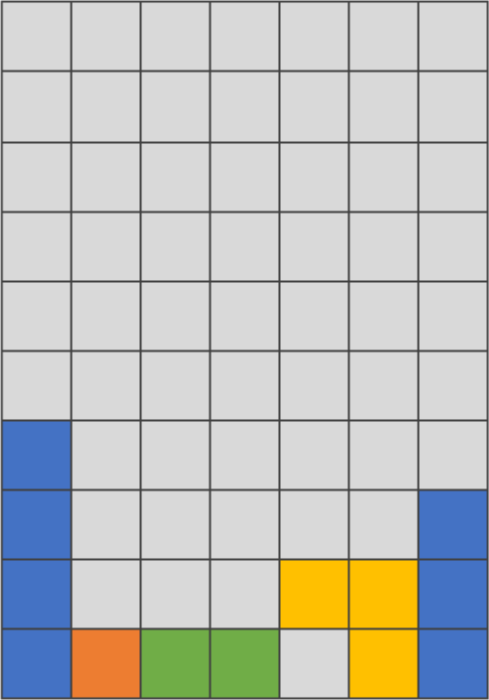
\includegraphics[width=0.8\linewidth]{tetris}
    %\vfill\null
    %\columnbreak

    \begin{lstlisting}
grid = {
  { 0, 0, 0, 0, 0, 0, 0 },
  { 0, 0, 0, 0, 0, 0, 0 },
  { 0, 0, 0, 0, 0, 0, 0 },
  { 0, 0, 0, 0, 0, 0, 0 },
  { 0, 0, 0, 0, 0, 0, 0 },
  { 0, 0, 0, 0, 0, 0, 0 },
  { 1, 0, 0, 0, 0, 0, 0 },
  { 1, 0, 0, 0, 0, 0, 1 },
  { 1, 0, 0, 0, 4, 4, 1 },
  { 1, 2, 3, 3, 0, 4, 1 }
};
    \end{lstlisting}
  \end{multicols}
  Die Aufgabe ist nun eine Methode zu schreiben, die die unterste Zeile löscht,
  falls sie ``voll'' ist.
  \begin{enumerate}[a)]
  \item Schreibe eine Methode \lstinline|bool is_last_line_complete()|, die prüft,
    ob die letzte Zeile des Grids gelöscht werden kann, d.\,h.\ prüft, ob diese
    Zeile nur nicht-null Einträge enthält. Die Größe des Spielfeldes kann dabei
    mit \lstinline|grid.rows()| bzw. \lstinline|grid.cols()| abgefragt werden.
  \item Schreibe nun eine Methode, die die letzte Zeile löscht. Dabei sollen einfach
    alle Zeilen darüber nach unten verschoben werden und die erste Zeile des
    Spielfelds mit Nullen gefüllt werden.
  \end{enumerate}
\end{exercise}

\begin{exercise}
  Diese Aufgabe beschäftigt sich mit sog. \emph{Monte Carlo Integration}. Ziel ist es
  die Zahl $\pi$ zu approximieren. Die Methode basiert auf folgender Idee:

  Generiert man $n$ zufällige Punkte in einem Quadrat der Länge $l$ und zählt dann die Punkte,
  die in diesem Quadrat in einem Kreis liegen, der den Durchmesser $l$ hat, dann gilt
  \begin{equation}
    \label{eq:mc}
    \lim_{n \rightarrow \infty} \frac{A_{\text{Kreis}}}{A_{\text{Quadrat}}} = \pi\,,
  \end{equation}
  wobei $A$ die Anzahl der Punkte innerhalb des Kreises bzw. des Quadrates angibt.
  In dieser Aufgabe soll eine Funktion geschrieben werden, die für gegebenes $n$ den
  Quotienten in~\eqref{eq:mc} berechnet. Als Quadrat wählen wir das Quadrat mit den
  Randpunkten $(-1,-1)\,,(-1,1)\,, (1,1)\,, (1,-1)$. Allerdings betrachten wir nur ein
  Viertel dieses Quadrats und multiplizieren später das Ergebnis einfach mit 4, siehe Abbildung:
  \begin{figure}[H]
    \centering
    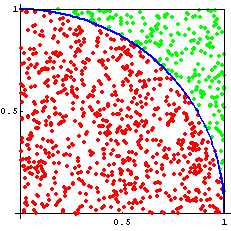
\includegraphics[width=0.55\textwidth]{montecarlo.png}
  \end{figure}
  Ziel ist es nun eine Funktion \lstinline|double pi_mc(int n)| zu schreiben, die nach dem
  obigen Prinzip $\pi$ approximiert. Gehe dazu folgendermaßen vor:
  \begin{itemize}
  \item Erzeuge $n$ zufällige Punkte im Einheitsquadrat (wie in der Abbildung oben).
    Es kann davon ausgegangen werden, dass eine Funktion \lstinline|randu(int a, int b)|
    existiert, die gleichverteilte Zufallszahlen im Intervall $[a,b]$ erzeugt.
  \item Zähle die Punkte, die innerhalb des Viertelkreises liegen (in der Abbildung rot). Hinweis:
    Der Kreis hat Radius 1. Der Abstand zweier Punkte $p_1 = (x_1, y_1)$ und $p_2 = (x_2, y_2)$ ist
    \[
      d(p_1, p_2) = \sqrt{{(x_1 - x_2)}^2 - {(y_1 - y_2)}^2}\,.
    \]
  \item Teile am Ende die Anzahl der Punkte im Kreis durch die Anzahl der insgesamt
    erzeugten Punkte und multipliziere das Ergebnis noch mit vier (s.o.).
  \end{itemize}
  
\end{exercise}

\end{document}

% Local Variables:
% End:
 